\documentclass[../main.tex]{subfiles}

\begin{document}

\subsection{Simulación de los circuitos RC y RL}
El primer paso a llevar a cabo en la implementación de las simulaciones de los circuitos RC y RL, será plantear un algoritmo que nos permita generar los datos correspondientes a cada una de las magnitudes físicas de ambos circuitos.\\ 

\subsubsection{Etapas del proceso}
Comenzamos entonces identificando cuáles son las etapas en las que podemos dividir el proceso de llevar a cabo una simulación:

\begin{itemize}
    \item En primer lugar tenemos la etapa de \textit{stop} en la que, como su propio nombre indica, el sistema se encuentra totalmente en reposo, pausando así los subprocesos de generación y representación de resultados. Por defecto, esta etapa será activada cada vez que se cree una nueva instancia de cualquiera de los dos circuitos. \\

    Dado que el proceso de la simulación se encuentra pausado en esta fase, para pasar a cualquiera de las otras (ver siguientes) el usuario debe de forzar al sistema utilizando el interfaz de usuario de la aplicación.

    \item La segunda etapa a destacar y que podriamos considerar como la principal, consta de un subproceso cíclico en el que se lleva a cabo la generación, el procesamiento y el almacenamiento de los datos; y paralelamente, su representación. Esta etapa estará activa siempre y cuando la simulación no haya finalizado por alguna de las siguientes causas: el circuito a simular no haya alcanzado su estado de equilibrio y por lo tanto, no tiene sentido seguir generando resultados; se haya cumplido alguna de las restricciones impuestas por el usuario; o bien, la simulación haya sido reiniciada manualmente. Este último caso es algo especial, el cuál veremos en el siguiente punto. \\

    A esta etapa del proceso de la simulación la denominaremos etapa activa o \textit{running}.

    \item Como hemos comentado anteriormente, es posible reiniciar la simulación de forma manual, iniciando entonces la etapa de \textit{reload} o reinicio. En ella se hace una limpieza de todos los resultados que se han ido generando previamente y justo después, se vuelve a iniciar la simulación del último circuito establecido, volviendo así a la etapa de \textit{running}. 

    \item Por último, tenemos el subproceso de cambiar de valor un componente del circuito. Aunque esta no será considerada como una etapa más del proceso sino más bien como un paso intermedio entre la  
    simulación de dos circuitos diferentes ya que en este no se actúa directamente sobre los resultados de la simulación actual, cabe destacar que al igual que al igual que la etapa de \textit{reload}, se trata de un subproceso donde la finalización de este no depende del usuario, sino del propio flujo del sistema. 
    
   
\end{itemize}

Para comprender mejor el funcionamiento global de la simulación, se ha elaborado el diagrama de la figura \ref{fig::diagrama-algoritmo}, en el que se puede ver con mayor detalle la interacción entre los diferentes subprocesos.\\


\begin{figure}[!h]
    \centering
    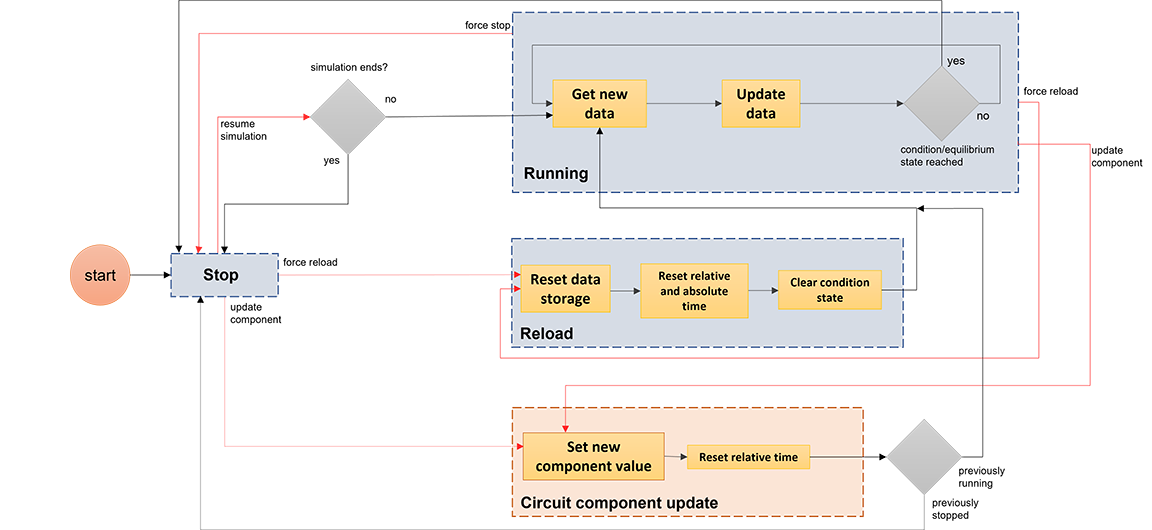
\includegraphics[width=\textwidth]{images/diagrama-algoritmo.png}
    \caption{Representación abstracta la aplicación. Las flechas en \textit{rojo} indican las acciones que el usuario puede tomar sobre la aplicación; en \textit{negro} las acciones que toma el sistema por su cuenta. }
    \label{fig::diagrama-algoritmo}
\end{figure}

 A continuación presentamos los aspectos más importantes de las simulaciones, en los que trataremos conceptos como \textit{ventana de datos} o \textit{condiciones de parada}.


\subsubsection{Generación de datos}
Que el sistema se encuentre en las etapas de \textit{stop} o \textit{reload} depende más de las acciones que tome el usuario de la aplicación que del propio flujo del proceso, por lo que nos centraremos en la etapa activa para la generación de datos en tiempo real. Nos apoyeremos entonces en el método \textit{componentDidMount} del componente de la simulación, que como ya sabemos, solamente se ejecuta una vez durante la vida de un componente (concretamente durante su creación). \\

Aprovechando la capacidad de JavaScript para crear funciones privadas en el cuerpo de otros métodos y funciones, crearemos la instancia de una nueva función local y asíncrona dentro del procedimiento \textit{componentDidMount}, la cuál se ejecutará repetitivamente cada cierto tiempo, como por ejemplo cada 150 milisegundos. A estas funciones también se le conocen como \textit{setInterval}. La elección del valor de este intervalo se toma en base a la velocidad de generación de los datos que queramos. Si este es muy grande, el tiempo de espera entre la producción de dos valores crece demasiado, ralentizando así la representación de los mismos; pero si es muy pequeño, la cantidad de información generada podría llegar a ser demasiado grande, pudiendo llegar a colapsar la propia aplicación. Frente a las alternativas que presenta este dilema nos quedamos con la segunda opción, pues podemos hacer uso de una \textit{ventana de datos} de longitud fija para almacenar los resultados.

Por cada magnitud física a representar, utilizaremos una ventana de datos diferente. Se trata de una lista de longitud no variable sobre la que debemos de controlar la inserción de nuevos resultados. Cuando el número de datos de la ventana es inferior a su longitud no existe ningún problema, pues podemos ir añadiendo otros  nuevos al final de la misma y mantener así el orden de producción (figura \ref{fig::ventana_datos_1}). Sin embargo, si excedemos el límite, lo que haremos será eliminar el de mayor antigüedad, desplazando el resto una posición hacia la izquierda (\textit{shift}) y obteniendo así un hueco libre para añadir nueva información (figura \ref{fig::ventana_datos_2}). El objetivo de esto no es otro que mantener el orden de llegada para que la representación de los resultados sea lo más cómoda posible. \\


\begin{figure}[!h]
    \centering
    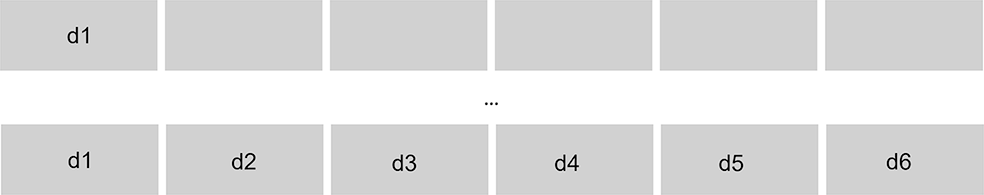
\includegraphics[width=0.9\textwidth]{images/ventana_datos_1.png}
    \caption{Cada que generamos un nuevo resultado y aún queda espacio libre, este se añade al final de la lista, respetando así el orden en el que fueron generados.}
    \label{fig::ventana_datos_1}
\end{figure}

\begin{figure}[!h]
    \centering
    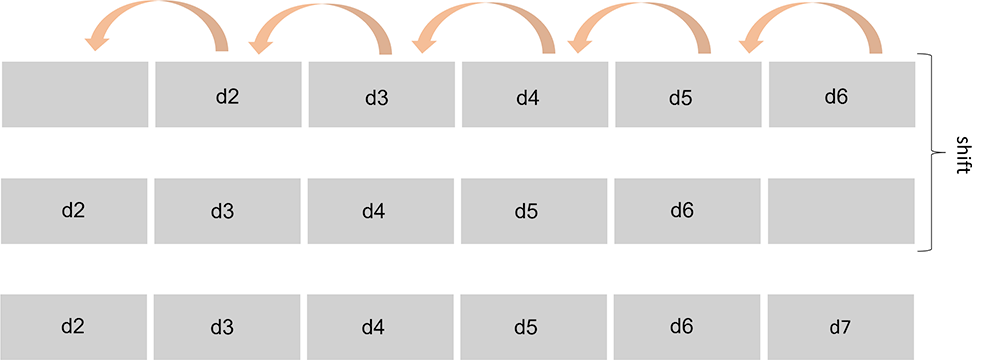
\includegraphics[width=\textwidth]{images/ventana_datos_2.png}
    \caption{Cuando ya no queda hueco libre en la ventana de datos, realizamos un \textit{shift} de esta lista, dejando así espacio libre para la insercion de nuevos resultados.}
    \label{fig::ventana_datos_2}
\end{figure}

Además, las funciones del tipo \textit{setInterval} retornan un valor identificativo que hacen referencia al temporizador de la función. Este será utilizado por el componente asociado al simulador en su etapa de destrucción para eliminar la llamada reiterativa de este proceso. Y aunque realmente esta limpieza no es necesaria (ya que solamente tendremos una función de este tipo ejecutándose al mismo tiempo), si que es de buena práctica llevarla a cabo, pues si el número de funciones \textit{setInterval} utilizadas es mayor puede causar problemas de rendimiento en la aplicación si no se toman este tipo de medidas.\\

\subsubsection{Tiempo absoluto y tiempo relativo de la simulación}
Por otro lado, para garantizar la correcta visualización de los datos correspondientes a cada una de las magnitudes físicas en las gráficas, tenemos que considerar dos valores de tiempo diferentes, los cuales vamos a denominar como \textit{tiempo absoluto} y \textit{tiempo relativo} de la simulación.\\

El primero de ellos, al que hemos llamado como \textit{tiempo absoluto}, será de utilidad para la representación de cada una de las magnitudes en un mismo eje. Como es lógico, esta variable de tiempo se verá incrementada a medida que se van obteniendo nuevos resultados de la simulación, tomando solamente valor nulo cuando se cree por primera vez la instancia del circuito o bien, la simulación sea reiniciada manualmente por el usuario en la etapa de \textit{reload}. 

Sin embargo, para calcular los resultados de cada una de las magnitudes físicas que describen el circuito en un instante de tiempo determinado, utilizaremos el \textit{tiempo relativo} de la simulación, el cuál tomará siempre valor cero cada vez que alguno de los componentes del circuito sea alterado y que se verá incrementado a la par que lo hace la variable de \textit{tiempo absoluto}.\\

De esta manera, utilizando una variable para el tiempo relativo podremos obtener los resultados de la simulación utilizando las expresiones del modelado en un instante de tiempo determinado y, al mismo tiempo, dicho valor lo almacenaremos con el valor de la variable de tiempo absoluto de la simulación. Esto permite visualizar en un mismo eje los resultados obtenidos de varias simulaciones, facilitando así la comparación entre ellos. Por ejemplo, en la figura \ref{fig::tiempos_simulacion} podemos observar con más detalle el uso de cada una de estas variables durante la simulación de un circuito RC, en el que vemos la evolución de la carga de un condensador cuando pasamos de una fuente de $12V$ a una de $6V$.\\




 \begin{figure}[!h]
        \centering
                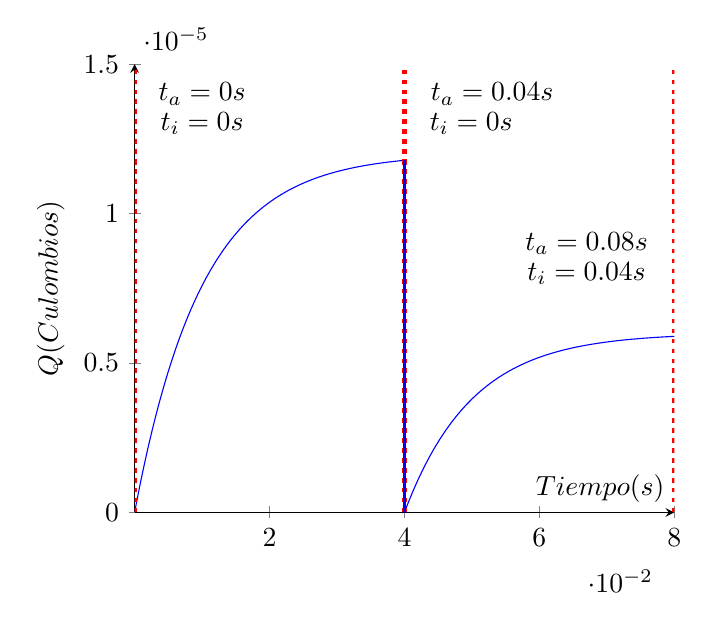
\begin{tikzpicture}
            \begin{axis}[
                axis y line = left,
                axis x line = middle,
                xmin=0,
                ymin=0, 
                xlabel = \(Tiempo (s)\),
                ylabel = {\(Q (Culombios)\)},
            ]
            %Below the red parabola is defined
            \addplot [
                domain=0:0.04, 
                samples=1000, 
                color=blue,
            ]
            {0.000012*(1-exp(-x/0.01))};
             
            \addplot [
                domain=0:0.08, 
                samples=100, 
                color=blue,
            ]
            {0.000006*(1-exp((-x + 0.04)/0.01))};

            %% Vertical line
            \addplot[ultra thick, dotted, samples=50, smooth, domain=0:0.08, red] coordinates {(0.04,0)(0.04, 0.000015)};
            
            \addplot[thick, samples=50, smooth, domain=0:0.08, blue] coordinates {(0.04,0)(0.04, 0.00001178)};

            \node[inner sep=1pt,] (0.04) at (0.0499,0.000013) {$t_i = 0s$};
            \node[inner sep=1pt,] (0.04) at (0.053, 0.000014) {$t_a = 0.04s$};


            %% Vertical left line
            \addplot[ultra thick, dotted, samples=50, smooth, domain=0:0.08, red] coordinates {(0.08,0)(0.08, 0.000015)};
            \node[inner sep=1pt,] (0.08) at (0.067, 0.000008) {$t_i = 0.04s$};
            \node[inner sep=1pt,] (0.08) at (0.067, 0.000009) {$t_a = 0.08s$};

            %% Vertical left line
            \addplot[ultra thick, dotted, samples=50, smooth, domain=0:0.08, red] coordinates {(0,0)(0, 0.000015)};
            \node[inner sep=1pt,] (0) at (0.01, 0.000013) {$t_i = 0s$};
            \node[inner sep=1pt,] (0) at (0.01, 0.000014) {$t_a = 0s$};
            
        
        \end{axis}
        \end{tikzpicture}

        \caption{Ejemplo de cómo se vería la evolución de la carga de un condensador en una simulación del circuito RC, donde se aprecian los valores que toman tanto el \textit{tiempo absoluto} ($t_a$) como el \textit{tiempo relativo} ($t_i$) cuando pasamos de una fuente de $12V$ a una de $6V$.}

        \label{fig::tiempos_simulacion}
    \end{figure}


\subsubsection{Condiciones de parada y escala de tiempo}
Otro de los aspectos a tener en cuenta en la implementación es saber cuándo dar por finalizada la simulación de un circuito. Por defecto, una simulación termina cuando las magnitudes físicas del circuito alcanzan su valor máximo o mínimo, dependiendo de si estas son crecientes o no en el tiempo. Sin embargo, habrá ocasiones en las que nos interesará simular mientras se cumpla una restricción.\\ 

Por un lado tenemos el circuito RC, el cuál lo estudiamos según la carga eléctrica que tiene el condensador; mientras que el circuito RL, lo hacemos según la intensidad de corriente que circula por él. Podríamos establecer restricciones como el porcentaje máximo de carga que alberga el condensador, la intensidad de corriente máxima que atraviesa a la resistencia o la cantidad de campo magnético creado en la bobina; no obstante, en todas ellas se nos va a presentar el problema de la figura \ref{fig::condicion-parada-1}. Tenemos la siguiente información:

\begin{itemize}
    \item Los resultados esperados, representados mediante líneas verticales y discontinuas. 
    
    \item Los resultados obtenidos, mostrados mediante las líneas de color azul y naranja.
    
    \item Error cometido, representado mediante una línea horizontal de color rojo.
\end{itemize}

El objetivo en la implementación de estas restricciones es minimizar el error que se ha cometido en la generación de datos. Para ello, debemos de utilizar una escala de tiempo lo suficientemente pequeña para que el ajuste sea el adecuado, y que además, permita generar una cantidad conveniente de datos y que así las curvas características de cada una de las magnitudes puedan apreciarse correctamente (figura \ref{fig::condiciones-de-parada}).\\ 

\begin{figure}[!h]
    \centering
    \subfloat[Escala de tiempo: 10s]{
        \label{fig::condicion-parada-1}
        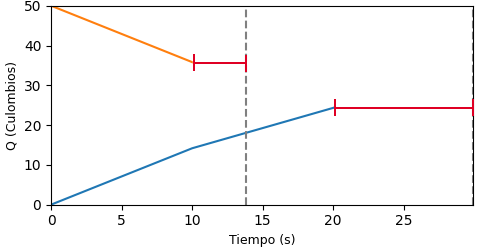
\includegraphics[width=0.45\textwidth]{images/carga-condicion-3.PNG}
    }
    \quad
    \subfloat[Escala de tiempo: 1s]{
        \label{fig::condicion-parada-2}
        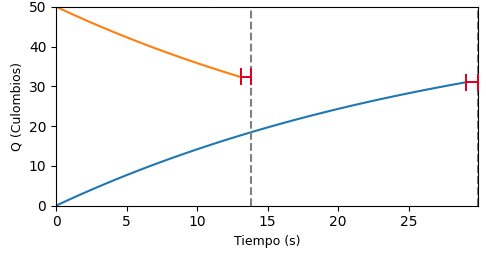
\includegraphics[width=0.45\textwidth]{images/carga-condicion-2.PNG}
    }


    \subfloat[Escala de tiempo: 1ms]{
        \label{fig::condicion-parada-3}
        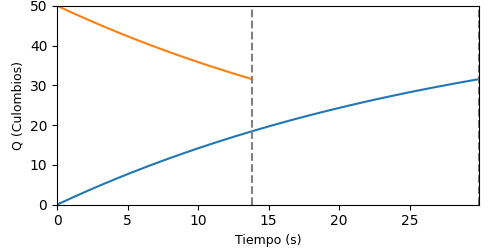
\includegraphics[width=0.45\textwidth]{images/carga-condicion-1.PNG}
    }
    \caption{Simulación de la carga del condensador bajo la condición de parada de que esta sea menor que el 63.08\% de su capacidad. En \textit{azul} se muestran los resultados obtenidos en estado de almacenamiento de energía; en \textit{naranja} en estado de disipación de energía.}

    \label{fig::condiciones-de-parada}
\end{figure}



Esto cuenta con un inconveniente y es que, cuanto menor sea la escala de tiempo utilizada mayor será el tiempo empleado en la generación de datos y por consiguiente, mayor tiempo se necesitará en mostrar los resultados. Así que para calcular dicha escala dependiendo de los valores de los componentes, utilizaremos la expresión que se muestra a continuación.

\begin{equation}
    t_{incremento} = 1 / t_{maximo}
    \label{eqq::tincremento}
\end{equation}

, dónde $t_{maximo}$ es la duración máxima de una simulación, la cuál puede tomar los siguientes valores:

\begin{itemize}
    \item En el caso del circuito RC, para resistencias del orden de $1K$, el tiempo máximo de simulación lo obtenemos al utilizar una resistencia de $9k \Omega$ y un condensador con la capacidad máxima permitida, en este caso de $100 \mu F$. Este tiempo es de 10 segundos. De igual forma para resistencias con un multiplicador de 1 mega ohmio, en concreto, con la resistencia de $9M \Omega$, el tiempo de la simulación asciende a 5700 segundos.
    
    \item En el circuito RL, ocurre lo contrario al anterior. Si para el circuito RC utilizamos el valor mínimo de la resistencia, ahora usaremos el máximo de la misma. Para resistencias de entre uno y nueve ohmios y una bobina con un coeficiente de autoinducción de $1H$, el tiempo de simulación máxima es de 5 segundos, mientras que para resistencias de uno a nueve kilo-ohmios, este tiempo será de 10 segundos.
\end{itemize}


Finalmente, para simplificar lo máximo posible la implementación de las condiciones de parada, se tendrá en cuenta como única condición el tiempo de simulación del circuito, ya que para la implementación de otras condiciones como la carga o la intensidad de corriente máximas, habría que calcular por un lado el tiempo que tardaría en alcanzar estos valores y posteriormente, una escala de tiempo adecuada.






\subsection{Comparación de resultados}
Para comprobar que efectivamente los resultados que se están generando en la aplicación son realmente los esperados y se aproximan suficientemente a los reales, realizaremos un par de pruebas utilizando un \textit{script} de \textit{python} que hemos elaborado haciendo uso de librerías como \textit{numpy} \cite{numpy} y \textit{matplotlib} \cite{matplotlib}, las cuáles nos van a facilitar la creación de ejes cartesianos para mostrar los resultados de cada una de las magnitudes; además, añadiremos información adicional como el tiempo empleado en la simulación. Como es lógico; al igual que en la aplicación, en el \textit{script} deberemos de indicar además del valor de cada uno de los componentes y el tipo de circuito, la escala de tiempo a utilizar (ver tabla \ref{tab::argumentos-script} en el apéndice \ref{app::manual_instalacion}).\\ 

La ejecución de estas pruebas son prácticamente instantáneas, por lo que tenemos libertad en usar escalas de tiempo muy pequeñas sin ningún problema. Sin embargo, esto puede dar problemas de precisión, pues el tiempo empleado en la simulación del \textit{script} puede ser que no coincida con el de la aplicación; ya que al estar utilizando escalas de tiempo muy inferiores (o superiores dependiendo del caso) se pueden generar más o menos datos, mostrando así curvas más o menos precisas. 

Para abordar este problema utilizaremos la \textit{flag ``-t''} del programa en python. Esta nos permite indicar durante cuanto tiempo queremos obtener datos y plasmarlos en las gráficas que este genera, de tal forma que se prolonguen lo máximo posible en el tiempo acorde a los resultados de la aplicación; todo ello independientemente de la escala de tiempo utilizada.\\ 




Además, en todas las pruebas, la fuente a utilizar será de $6V$, al igual que en el laboratorio. También usaremos un condensador con $30 \mu F$ de capacidad, una bobina con un coeficiente de autoinducción de $1H$ (o $1000mH$ como se indica en la aplicación) y resistencias de $3\Omega$, $3k \Omega$ y $3M \Omega$, dependiendo del caso. 



\subsubsection{Caso de prueba 1: carga y descarga de un condensador}
La primera prueba que llevaremos a cabo será la carga y descarga de un condensador de $30 \mu F$ de capacidad, utilizando las resistencias de $3k\Omega$ y $3M\Omega$. \\

Introduciendo estos datos en la aplicación, obtenemos los resultados que se muestran en las figuras \ref{fig::caso_prueba_rc_1_app_carga} y \ref{fig::caso_prueba_rc_1_app_descarga}, para la carga y la descarga respectivamente. Utilizando el \textit{script} elaborado, las gráficas resultantes son las de la figura \ref{fig::caso_prueba_rc_1_res}, dónde la escala de tiempo establecida es de $1$ microsegundo, la cuál nos permite conseguir una mayor precisión.\\


\begin{figure}[!h]
    \centering
    \subfloat[Q(t) e I(t)]{
        \label{fig::caso_prueba_rc_1_app_1}
        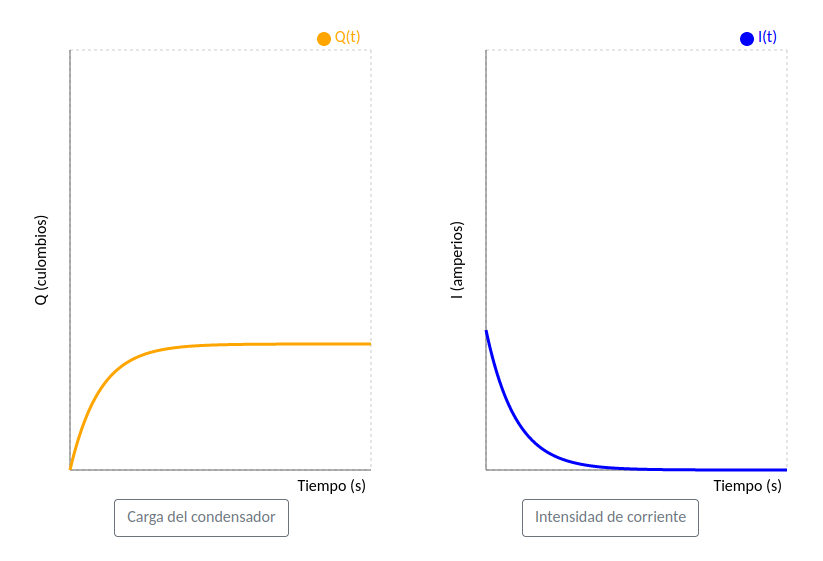
\includegraphics[width=0.5\textwidth]{images/caso_prueba_rc_1_app_1.png}
    }
    \quad
    \subfloat[$V_C(t)$ y $V_R(t)$]{
        \label{fig::caso_prueba_rc_1_app_2}
        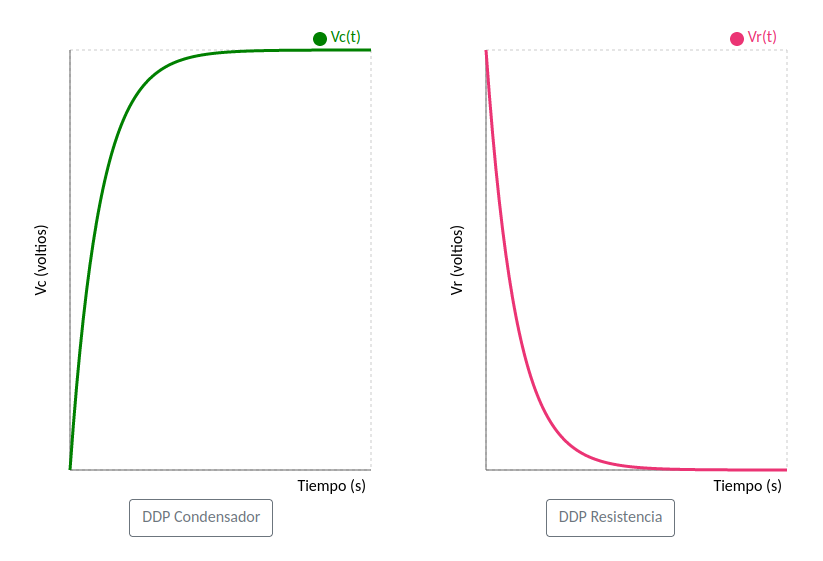
\includegraphics[width=0.5\textwidth]{images/caso_prueba_rc_1_app_2.png}
    }


    \subfloat[$E_e(t)$]{
        \label{fig::caso_prueba_rc_1_app_3}
        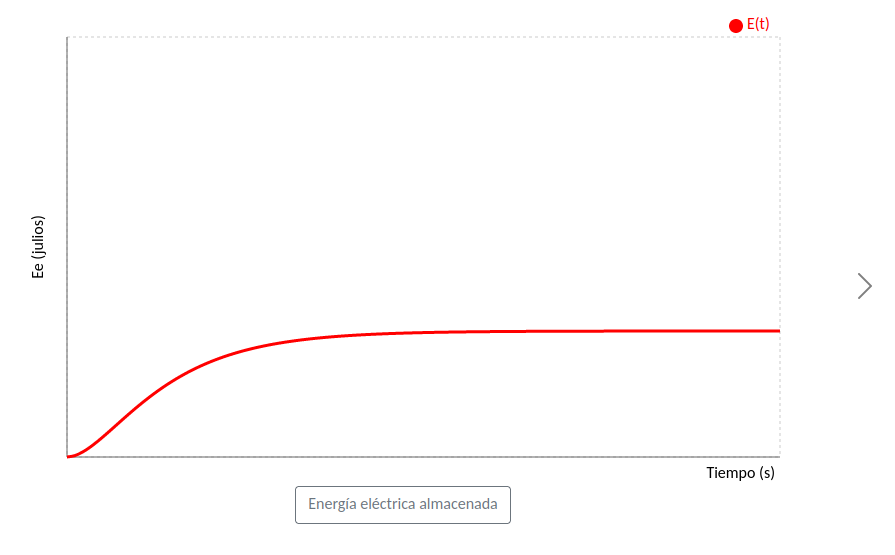
\includegraphics[width=0.5\textwidth]{images/caso_prueba_rc_1_app_3.png}
    }
    \caption{Resultados de la aplicación de una simulación del circuito RC en estado de carga, para una fuente de $6V$, una resistencia de $3k\Omega$ y un condensador de $30\mu F$.}

    \label{fig::caso_prueba_rc_1_app_carga}
\end{figure}


\begin{figure}[!h]
    \centering
    \subfloat[Q(t) e I(t)]{
        \label{fig::caso_prueba_rc_1_app_4}
        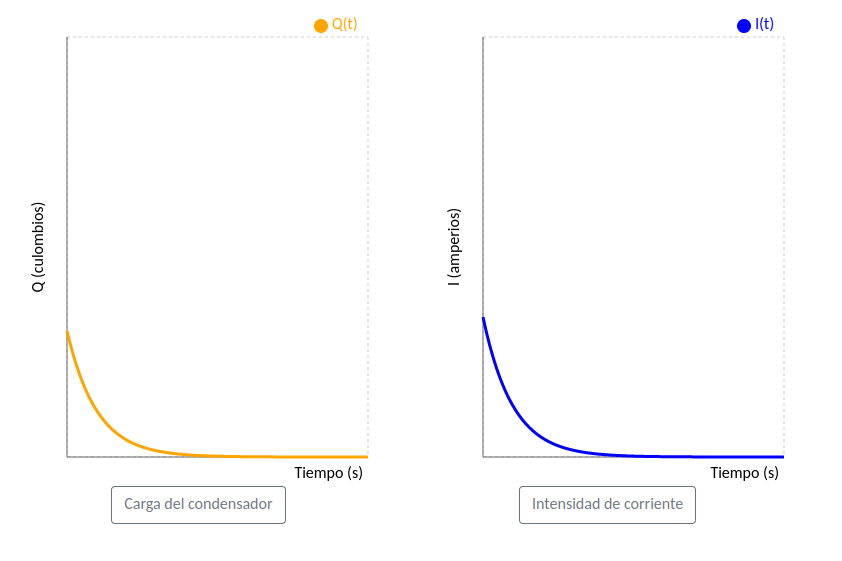
\includegraphics[width=0.5\textwidth]{images/caso_prueba_rc_1_app_4.png}
    }
    \quad
    \subfloat[$V_C(t)$ y $V_R(t)$]{
        \label{fig::caso_prueba_rc_1_app_5}
        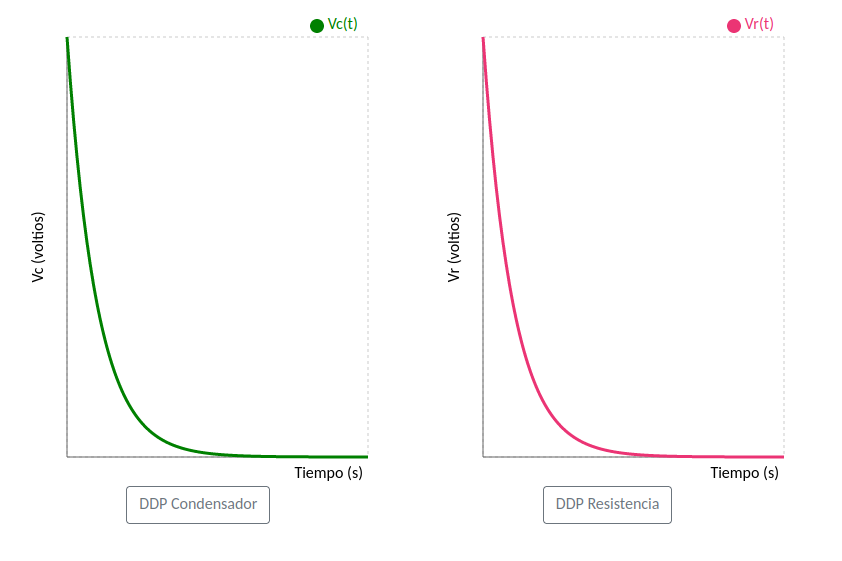
\includegraphics[width=0.5\textwidth]{images/caso_prueba_rc_1_app_5.png}
    }


    \subfloat[$E_e(t)$]{
        \label{fig::caso_prueba_rc_1_app_6}
        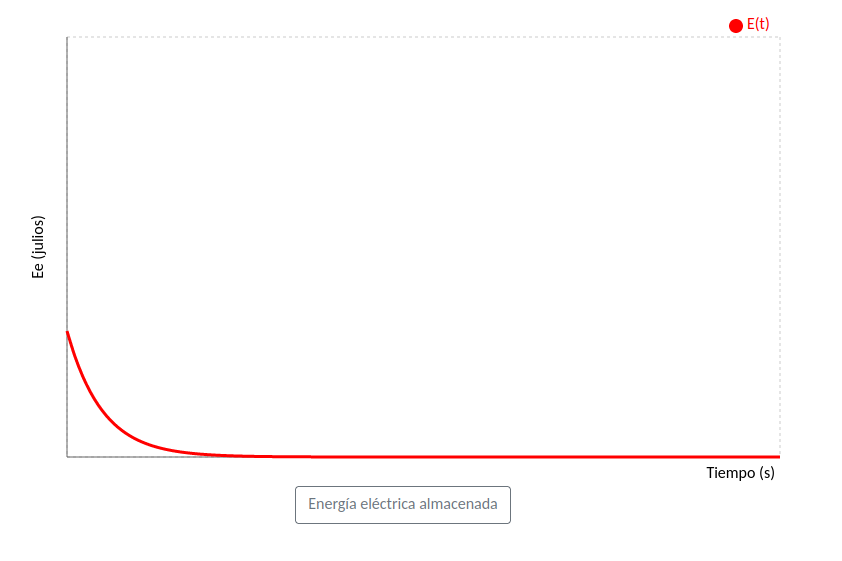
\includegraphics[width=0.5\textwidth]{images/caso_prueba_rc_1_app_6.png}
    }
    \caption{Resultados de la aplicación de una simulación del circuito RC en estado de descarga, para una fuente de $6V$, una resistencia de $3k\Omega$ y un condensador de $30\mu F$.}

    \label{fig::caso_prueba_rc_1_app_descarga}
\end{figure}

\begin{figure}[!h]
    \centering
    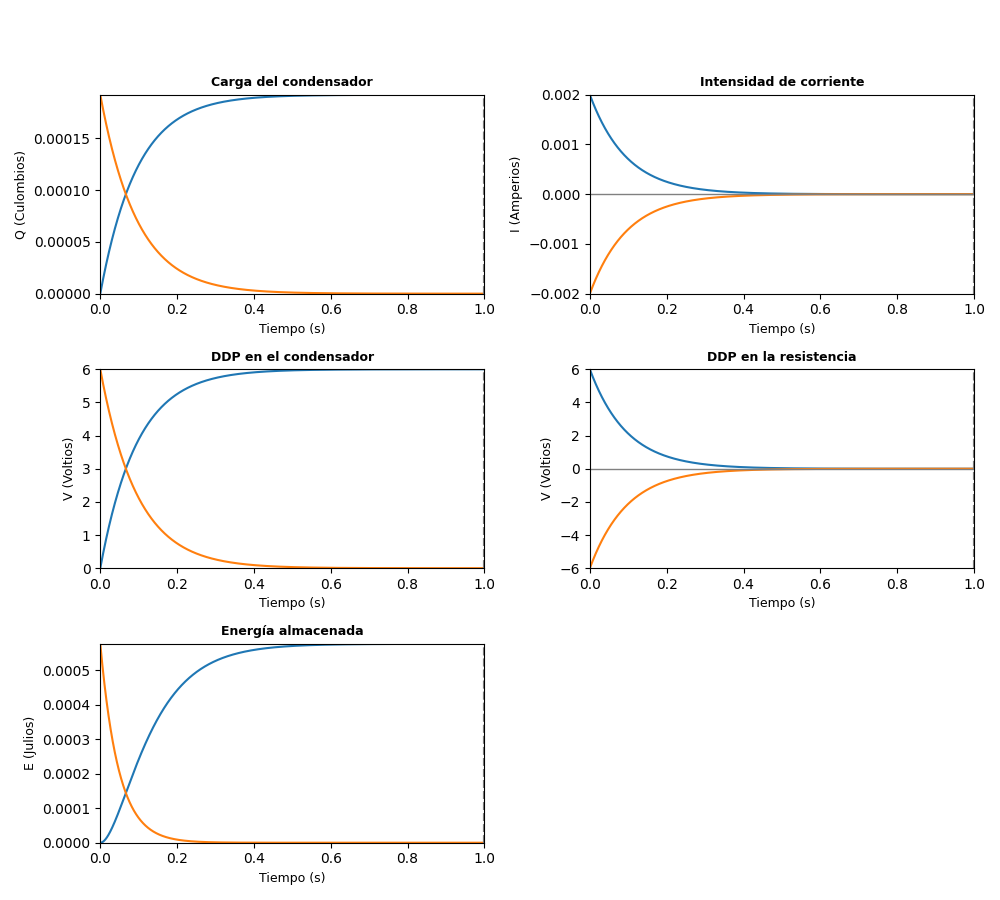
\includegraphics[width=0.8\textwidth]{images/caso_prueba_rc_1.png}
    \caption{Caso de prueba 1: carga y descarga de un condensador de $30\mu F$ de capacidad y una resistencia de $3k\Omega$.}
    \label{fig::caso_prueba_rc_1_res}
\end{figure}

Podemos observar que durante el estado de carga del condensador, tanto la energía en el mismo como la diferencia de potencial entre sus armaduras aumentan; por el contrario, la intensidad de corriente y por consiguiente el potencial eléctrico en la resistencia disminuyen hasta ser cero. Al contrario ocurre durante la descarga del condensador, dónde tanto la energía como el potencial eléctrico en este dispositivo disminuyen, de igual forma que lo hacen la intensidad de corriente y la diferencia de potencial de la resistencia.\\

A partir de aquí, podríamos jugar con el valor de la resistencia para cargar y descargar más o menos rápido el condensador; o bien, cambiar la capacidad de este dispositivo para almacenar mayor o menor energía.



\subsubsection{Caso de prueba 2: carga y descarga de un inductor}
La segunda prueba a realizar será la carga y descarga de un inductor con un coeficiente de autoinducción de $1H$, utilizando para ello una resistencia de $3\Omega$. \\

En las figuras \ref{fig::caso_prueba_rl_1_app_carga} y \ref{fig::caso_prueba_rl_1_app_descarga} podemos observar los resultados obtenidos mediante la aplicación; y en la figura \ref{fig::caso_prueba_rl_1_res}, las gráficas generadas por el \textit{script}, dónde la escala de tiempo a utilizar será de $1$ microsegundo.\\


\begin{figure}[!h]
    \centering
    \subfloat[I(t)]{
        \label{fig::caso_prueba_rl_1_app_1}
        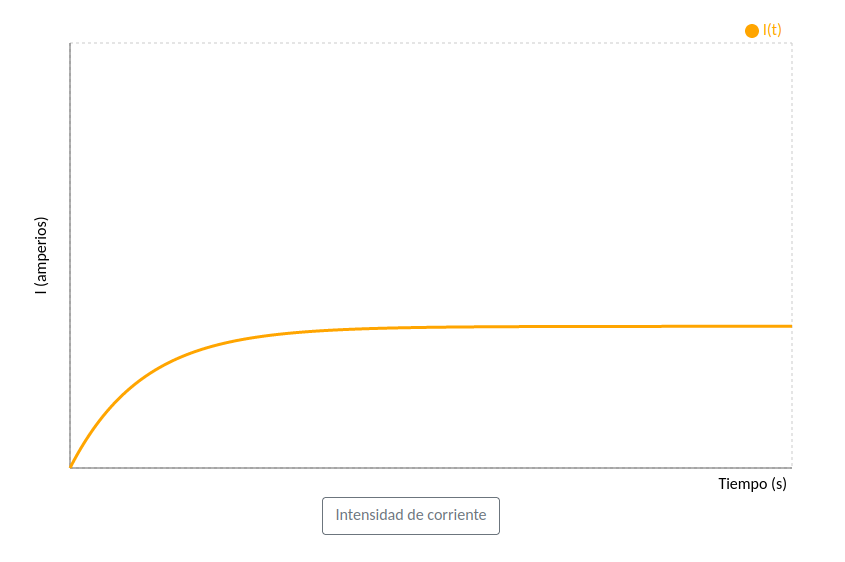
\includegraphics[width=0.5\textwidth]{images/caso_prueba_rl_1_app_1.png}
    }
    \quad
    \subfloat[$V_L(t)$ y $V_R(t)$]{
        \label{fig::caso_prueba_rl_1_app_2}
        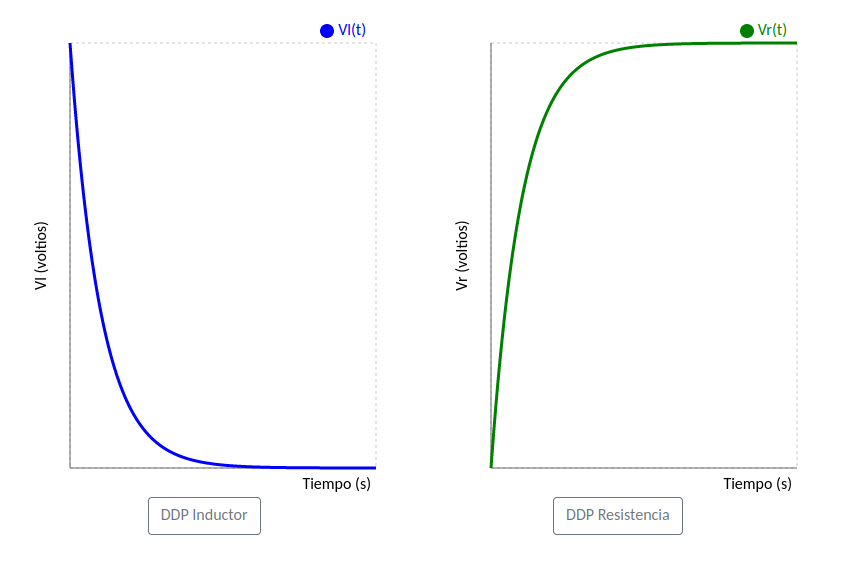
\includegraphics[width=0.5\textwidth]{images/caso_prueba_rl_1_app_2.png}
    }


    \subfloat[$E_e(t)$ y $\phi(t)$]{
        \label{fig::caso_prueba_rl_1_app_3}
        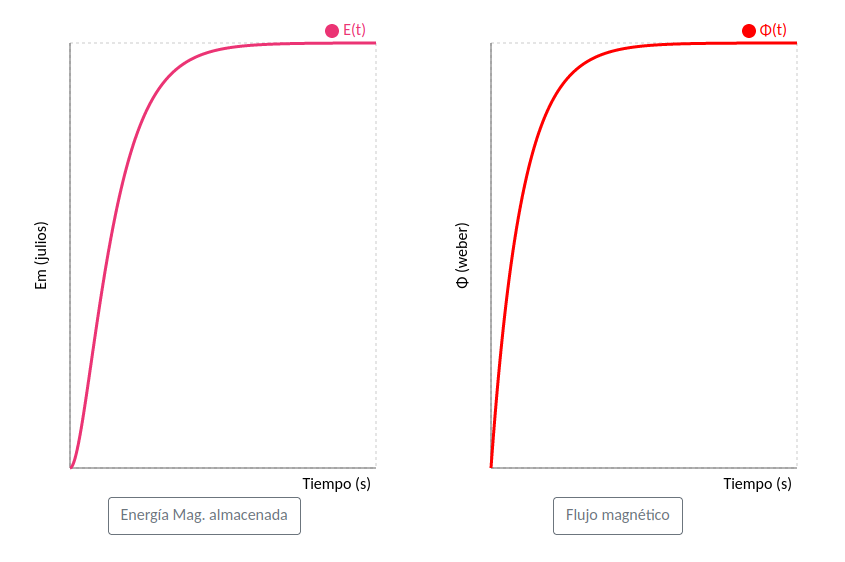
\includegraphics[width=0.5\textwidth]{images/caso_prueba_rl_1_app_3.png}
    }
    \caption{Resultados de la aplicación de una simulación del circuito RL en estado de almacenamiento de energía, para una fuente de $6V$, una resistencia de $3 \Omega$ y un inductor de $1H$.}

    \label{fig::caso_prueba_rl_1_app_carga}
\end{figure}


\begin{figure}[!h]
    \centering
    \subfloat[I(t)]{
        \label{fig::caso_prueba_rl_1_app_4}
        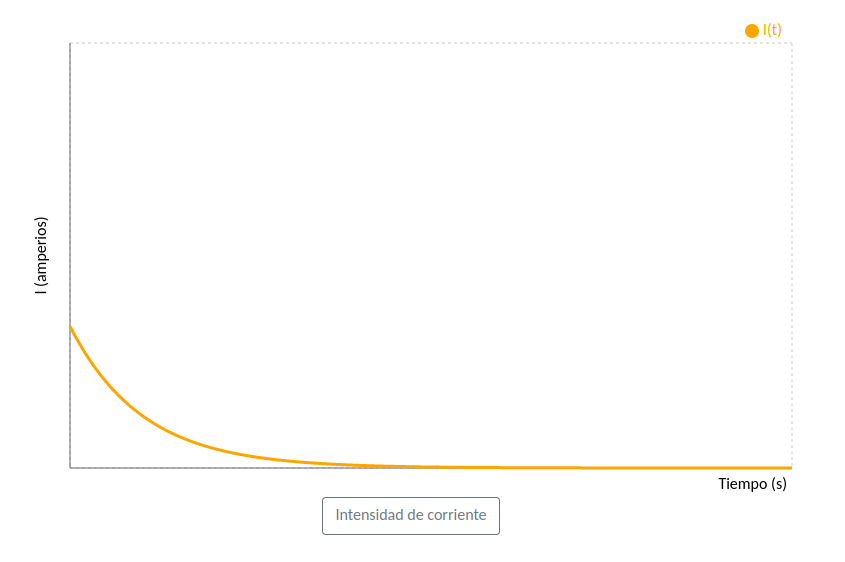
\includegraphics[width=0.5\textwidth]{images/caso_prueba_rl_1_app_4.png}
    }
    \quad
    \subfloat[$V_L(t)$ y $V_R(t)$]{
        \label{fig::caso_prueba_rl_1_app_5}
        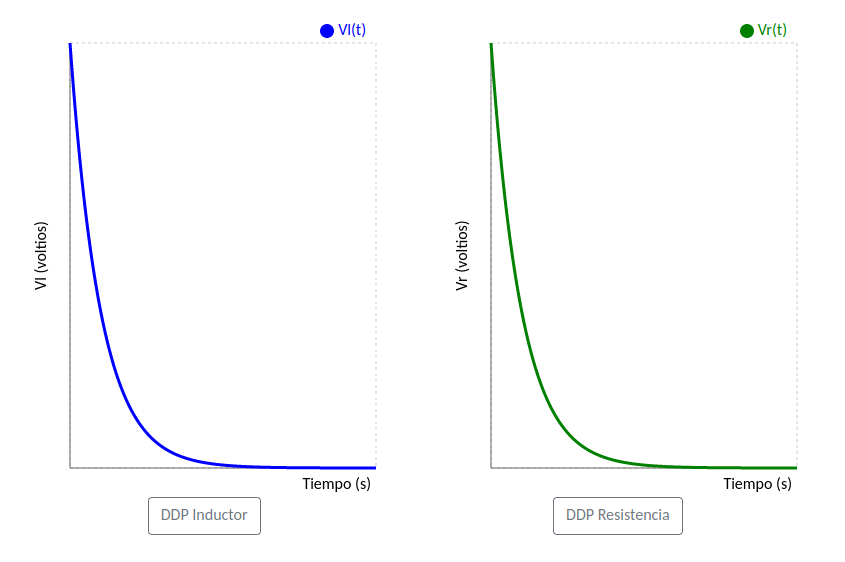
\includegraphics[width=0.5\textwidth]{images/caso_prueba_rl_1_app_5.png}
    }


    \subfloat[$E_e(t)$ y $\phi(t)$]{
        \label{fig::caso_prueba_rl_1_app_6}
        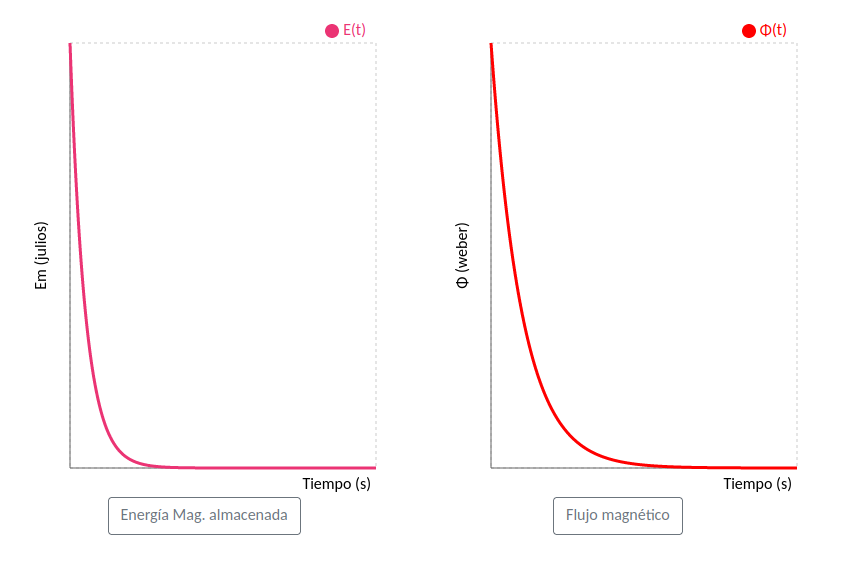
\includegraphics[width=0.5\textwidth]{images/caso_prueba_rl_1_app_6.png}
    }
    \caption{Resultados de la aplicación de una simulación del circuito RL en estado de disipación de energía, para una fuente de $6V$, una resistencia de $3 \Omega$ y un inductor de $1H$.}

    \label{fig::caso_prueba_rl_1_app_descarga}
\end{figure}


\begin{figure}[!h]
    \centering
    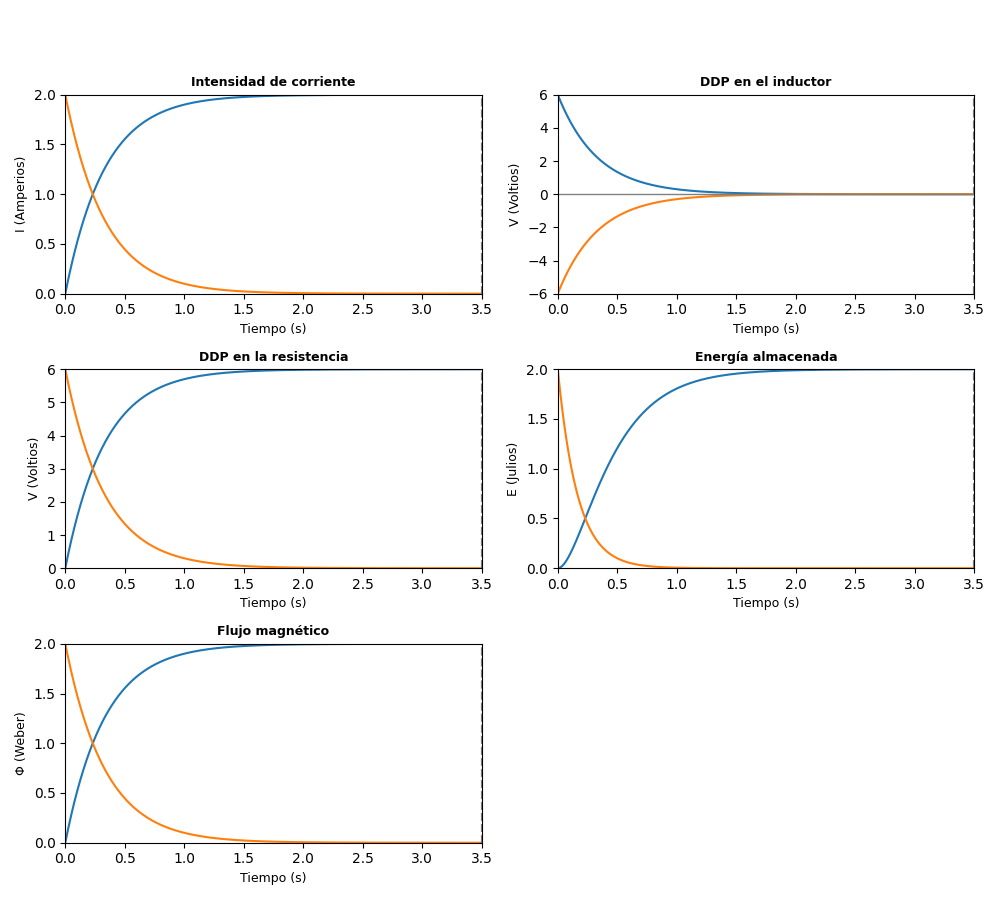
\includegraphics[width=0.8\textwidth]{images/caso_prueba_rl_1.png}
    \caption{Caso de prueba 2: carga y descarga de un inductor de $1H$ de coeficiente de autoinducción y una resistencia de $3 \Omega$.}
    \label{fig::caso_prueba_rl_1_res}
\end{figure}

Debido al fenómeno de autoinducción, observamos que la intensidad de corriente aumenta a medida que lo hace la cantidad de campo magnético en la bobina, al mismo tiempo que la energía y la diferencia de potencial en la resistencia. Durante el proceso de disipación de energía, la caída del campo magnético creado en el inductor causa un descenso en la intensidad de corriente (de nuevo por el fenómeno de autoinducción), reduciendo así los potenciales en el inductor y la resistencia hasta cero. \\

De igual forma, se podrían probar nuevos casos cambiando el valor de la resistencia y el coeficiente de autoinducción, y comprobar que efectivamente el tiempo que transcurre durante el almacenamiento y la disipación de energía magnética del inductor varía dependiendo de estos valores.\\



\end{document}